\documentclass[letterpaper]{article}

\usepackage{natbib,alifexi}
\usepackage{amsmath}
\usepackage[french]{babel}
\usepackage[utf8]{inputenc}
\usepackage{hyperref}
\usepackage{amsfonts}
\usepackage{graphicx}
\usepackage{blkarray}
\usepackage{tikz}
\usetikzlibrary{automata, positioning}

\newcommand{\colornode}[1][]{\node[state,
	    align=center,
	    text=gray!40!black,
	    draw=gray,
	    fill=gray!20!white,{#1}]}
\newcommand{\bigcolornode}[1][]{\node[state,
	    align=center,
	    text=gray!40!black,
	    draw=gray,
	    fill=gray!20!white,
	    text width=1.7cm,{#1}]}

\newcommand{\drawedge}{\draw[every loop, line width=0.4mm, fill=gray, draw=gray]}

\newcommand*{\fullref}[1]{\hyperref[{#1}]{\autoref*{#1} \nameref*{#1}}}


\title{Etude du Monopoly via les chaînes de Markov}
\author{Rémy Detobel\\
Mickael Randour\\
\mbox{}\\
Université Libre de Bruxelles, Bruxelles, Belgique \\
rdetobel@ulb.ac.be}


% =-=-=-=-=-=-=-=-= TODO GENERAL =-=-=-=-=-=-=-=-=
% - Bibliographie (revoir l'affichage, la mise en page)
% - Résultats
% - Conclusion


\begin{document}
\maketitle

\begin{abstract}
  Modélisation et étude du Monopoly à travers les chaînes de Markov.
  Les concepts principaux de ce modèle qu'est une chaîne de Markov,
  seront présentés et expliqués.  Les différents choix permettant 
  d'adapter le Monopoly afin qu'il puisse être modélisé comme une chaîne 
  de Markov seront également expliqués.  Enfin, une description de 
  l'application et des résultats récupérés par l'implémentation de cette 
  modélisation sera également faite et permettra de déterminer les cases 
  les plus fréquentés ainsi que les cases les plus rentables.
\end{abstract}

%%%%%%%%%%%%%% SECTION %%%%%%%%%%%%%%
\section{Introduction}
  Contrairement aux idées reçues, chaque case du Monopoly n'a pas la même
  probabilité d'être visitée.  Il est donc intéressant d'étudier quels sont
  les cases les plus fréquentés mais également quels seraient les cases
  les plus rentables.  Dans cette idée, il est possible de modéliser
  le Monopoly à travers les chaînes de Markov.  Mais avant cela, il est 
  important de bien définir les chaînes de Markov ainsi que leurs propriétés.
  Les explications concernant ce modèle sont en grande partie basées 
  sur le cours de \citet{COURS}.
  Pour pouvoir modéliser le Monopoly comme étant une chaîne de Markov, 
  les règles du jeu doivent être clairement définies et des choix doivent
  être faits.  Ceux-ci seront donc expliqués et justifiés dans cet article.
  Les résultats trouvés suite à cette modélisation seront présentés afin
  de trouver, au final, les cases les plus visitées mais également les cases
  les plus rentables.
  % TODO ajouter des informations à l'intro (peut être plus conséquent)
  
  
%%%%%%%%%%%%%% SECTION %%%%%%%%%%%%%%
\section{Approche théorique}
  
  \subsection{Les chaînes de Markov}
    \label{def_chaine_markov}
    Une chaîne de Markov est une structure de données qui permet de modéliser l'évolution
    de l'état d'un système aléatoire.  Les chaînes de Markov sont basées sur le 
    fait que l'état actuel du système dépend uniquement de l'état précédent.
    Cette propriété peut être appelé ``propriété de Markov''.  Une chaîne de
    Markov est donc composée d'états et de liens entre ses différents états caractérisés
    par une certaine probabilité de passer d'un état A à un état B.
    Cette probabilité sera décrite plus en détail dans le point \ref{probabilite}.
    Il est possible de représenter une chaîne de Markov de plusieurs manières différentes.
    Dans la litérature (comme par exemple dans le cours \citet{COURS}), on utilisera 
    plus souvant la notation matricel, qui définit la chaîne de Markov $\mathcal{M}$ 
    tel que:
    $$\mathcal{M} = (S, \mathbf{P}, \iota_{init})$$
    Où $S$ représente l'ensemble de tous les états possibles, $\mathbf{P}$ une matrice $S \times S$
    où chaque élément est compris entre 0 et 1 et où cette valeur représente la probabilité 
    de passer d'un état à un autre (respectivement, l'état correspondant à la ligne et à la colonne).
    On appelera cette matrice $\mathbf{P}$ la \textit{matrice de transition}.
    $\iota_{init}$ est une matrice colonne où chaque ligne représente un état et la valeur
    associée représente la probabilité de commencer par cet état.  On peut retrouver d'autres
    variables dans la litérature (comme $AP$ et $L$ par exemple pour associer des propositions 
    atomiques aux états) mais celles-ci ne seront pas utiles dans cet article.
    Il est également possible de représenter une chaîne de Markov sous forme
    d'un graphe dirigé où chaque noeud représente un état et chaque arrête est pondéré
    en fonction de la probabilité de passer d'un état à un autre.
    Nottons également que les chaînes de Markov peuvent être utilisée
    dans un temps discret ou dans un temps continu.  Cependant, la modélisation
    du Monopoly n'inclura pas de temps continu et cet article traitera donc uniquement
    du temps discret.
    % TODO voir pour définir AP et L en 2 phrases
    
  \subsection{Exemple de chaîne de Markov}
    Afin d'illustrer les notions liées aux chaînes de Markov, cet article se 
    basera sur un exemple représentant les différents état que peut avoir 
    un avion.  On va donc ici considérer qu'un avion pourra avoir 6 états 
    différents: \textit{en vol} (noté \textit{vol}), \textit{attérissage} 
    (noté \textit{att.}), \textit{décollage} (noté \textit{dec.}), 
    \textit{au sol}, \textit{contrôle} (noté \textit{ctr.})
    et \textit{hors service} (noté \textit{h.s.}).
    On va considérer que lors de l'\textit{attérissage}, il y a une chance sur 
    3 pour qu'un voyant indique au pilote qu'un \textit{contrôle} est 
    nécessaire. On remarque également qu'il y a une chance sur 10 que 
    l'avion ne passe pas le \textit{contrôle} et soit considéré comme 
    \textit{hors service}.  On considèrera également que tous les avions commencent
    avec l'état \textit{au sol}.
    
    \subsubsection{Représentation matriciel}
      Comme vu au point \ref{def_chaine_markov}, il est possible de représenter une
      chaine de Markov comme étant:
      $$\mathcal{M} = (S, \mathbf{P}, \iota_{init})$$
      Pour notre exemple on aura donc:
      $$S = \{vol, dec., att., sol, ctr., h.s.\} $$
      $$ \mathbf{P} = 
	\begin{blockarray}{ccccccc}
	& vol & dec. & att. & sol & ctr. & h.s. \\
	  \begin{block}{c(cccccc)}
	    vol  & 0 & 0 & 1 & 0    & 0   & 0    \\
	    dec. & 1 & 0 & 0 & 0    & 0   & 0    \\
	    att. & 0 & 0 & 0 & 2/3  & 1/3 & 0    \\
	    sol  & 0 & 1 & 0 & 0    & 0   & 0    \\
	    ctr. & 0 & 0 & 0 & 9/10 & 0   & 1/10 \\
	    h.s. & 0 & 0 & 0 & 0    & 0   & 1    \\
	  \end{block}
	\end{blockarray}
      $$
      $$\iota_{init} = 
	\begin{blockarray}{cc}
	  \begin{block}{( c ) c}
	    0 & vol \\
	    0 & dec.\\
	    0 & att.\\
	    1 & sol\\
	    0 & ctr.\\
	    0 & h.s.\\
	  \end{block}
	\end{blockarray}
      $$
      
    \subsubsection{Représentation graphique}
      Il est également possible de représenter cette chaîne de Markov comme
      état un graphe dirigé (cfr point \ref{def_chaine_markov}):
      \begin{center}
	\begin{tikzpicture}
	  % Draw the states
	  \colornode[text width=1.7cm] (vol) {En vol};
	  
	  \colornode[below left=of vol] (att) {Attérissage};
	  \bigcolornode[below right=of vol] (dec) {Décollage};
	  
	  \bigcolornode[below right=of att] (sol) {Au sol};

	  \bigcolornode[below left=of sol] (ctr) {Contrôle};
	  \colornode[right=of ctr] (hs) {Hors service};

	  % Connect the states with arrows
	  \drawedge
	    (vol) edge[bend right, auto=right] node {1} (att)
	    (dec) edge[bend right, auto=right] node {1} (vol)
	    (sol) edge[bend right, auto=right] node {1} (dec)
	    (att) edge[bend right, auto=right] node {2/3} (sol)
	    (att) edge[bend right, auto=right] node {1/3} (ctr)
	    (ctr) edge[bend right, auto=left] node {9/10} (sol)
	    (ctr) edge[bend right, auto=right] node {1/10} (hs)
	    (hs) edge[loop right] node {1} (hs);
	  \draw [->, line width=0.4mm, fill=gray, draw=gray] (1.6,-5.4) -- (sol);
	\end{tikzpicture}
      \end{center}
    
  \subsection{Probabilité}
    \label{probabilite}
    La notion de probabilité peut se définir de plusieurs manières différentes 
    et de nombreux ouvrages (comme par exemple celui de \citet{IP}) décrivent 
    de manière très détaillé la notion de probabilité.  Dans ces ouvrages, on
    traite souvant des espaces de probabilité, qui demandent une approche très 
    abstraite et rigoureuses.  Cependant dans cet article, l'approche
    fréquentielle inspirée des statitistiques est suffisante.
    On définit donc la probabilité d'un événement aléatoire par la limite
    de la fréquence d'occurence d'un événement pour un nombre d'expériences
    tendant vers l'infini.  De manière plus formel, on peut décrire ce
    comportement comme $X$ étant une expérience aléatoire ayant
    $$X_i \mid i \in I $$
    pour résultats possibles, avec $I$ un ensemble d'indices (qui peuvent 
    être fini, infini dénombrable ou infini non-dénombrable).  On définit
    la probabilité du résultat $X_i$ pour $i \in I$ par:
    $$\lim_{n \to \infty}\frac {X_i(n)}n,$$
    avec $X_i(n)$, le nombre d'occurences du résultat $X_i$ lors de
    $n$ itérations de l'expérience $X$.  On note cette valeur
    $\mathbb P[X = X_i]$, si cette limite existe.
    % QUESTION Randour: ajouter ceci ?
    % Remarque : il est important de demander que la limite existe, par exemple 
    % si le nombre d'occurrences est sous la forme $X(n) = n\cos(n)$, on remarque 
    % qu'il est impossible de définir une probabilité, alors qu'une fréquence a un sens.
    
  \subsection{Simuler les changements d'état}
    Une chaîne de Markov permet donc d'estimer la probabilité de l'état
    future d'un système uniquement en se basant sur l'état actuel du système.
    Dans cette idée, la matrice de transition $\mathbf{P}$ représente tous les
    déplacements d'une unité possibles.  Si maintenant on veut connaitre
    les états accèssibles depuis notre état actuel après deux unités de temps,
    il suffit d'élevé la matrice de transition au carré.  Si l'on reprend
    notre exemple, on aura donc:
    \begin{align*}
    \mathbf{P}^2 &= 
      \begin{pmatrix}
	0 & 0 & 1 & 0    & 0   & 0    \\
	1 & 0 & 0 & 0    & 0   & 0    \\
	0 & 0 & 0 & 2/3  & 1/3 & 0    \\
	0 & 1 & 0 & 0    & 0   & 0    \\
	0 & 0 & 0 & 9/10 & 0   & 1/10 \\
	0 & 0 & 0 & 0    & 0   & 1    \\
      \end{pmatrix}^2\\
      &= 
      \begin{pmatrix}
        0 & 0    & 0 & 2/3  & 1/3 & 0    \\
	0 & 0    & 1 & 0    & 0   & 0    \\
	0 & 2/3  & 0 & 3/10 & 0   & 1/30 \\
	1 & 0    & 0 & 0    & 0   & 0    \\
	0 & 9/10 & 0 & 0    & 0   & 1/10 \\
	0 & 0    & 0 & 0    & 0   & 1    \\
      \end{pmatrix}
    \end{align*}
    
    
  \subsection{Caractéristiques d'une chaîne de Markov}
    On peut remarquer que la somme de tous les éléments de chaque ligne de la
    matrice de transition font $1$.  Ce phénomène peut également être vu
    sur la représentation graphique de la chaîne de Markov où la somme de chaque
    arrête quittant un noeud (un état donc) vaut $1$.  Par exemple, si l'on se
    concentre sur l'état ``att.'' (sur la représentation matriciel il s'agit donc 
    de la 3ème ligne), on a bien: $2/3 + 1/3 + 0$ qui vaut bien $1$.  De manière 
    plus formel, cette caractéristique peut être notée tel que pour un état $s \in S$:
    $$\sum\limits_{s' \in S} \mathbf{P}(s, s') = 1$$
    Où $\mathbf{P}(s, s')$ représente la probabilité (présente dans la matrice de
    transition) de passe de l'état $s$ à l'état $s'$.  Cette caractéristique est
    toujours vrai par défintion d'une chaîne de Markov mais également par définition
    d'une probabilité.\\
    En effet, chaque ligne de la matrice représente tous les états accèssible depuis
    l'état correspondant à la ligne courante.  Cette corrélation est encore plus
    visible sur la représentation graphique où chaque arrête partant de l'état courrant
    est la représentation d'une valeur positive dans la matrice.  Ces valeurs 
    représente la probabilité d'aller d'un état à un autre.  Les arrêtes sur le
    graphique et les valeurs dans la matrice représente tous les états accèssible
    depuis l'état actuel.  Il est donc normal que la probabilité d'aller de l'état
    actuelle à n'importe quel autre état de la chaine de Markov ait une probabilité de 1.\\
    Avec ce même raisonnement, il est logique de se rendre compte que la matrice
    de distribution initiale:
    $$\sum\limits_{s \in S} \iota_{init}(s) = 1$$
    
  \subsection{Comportement des chaînes des Markov}
    % ROBIN
% Pour composé connexe, habituellement, en français on parle de composante connexe, ni composé, ni composant. ;)

% Sinon j'ai un souci avec ta définition de SCC : elle laisse sous-entendre qu'il n'y a qu'une seule SCC (quote: un ensemble $T$ est un composé fortement connexe s'il est le plus grand ensemble [...]), or le principe de composate fortement connexe, c'est qu'il n'y en a qu'une seule si et seulement si le graphe est fortement connexe. Mais s'il ne l'est pas, alors il y a plusieurs SCCs.
% 
% La définition usuelle d'une composante (fortement) connexe est la suivante (pour $Q$ l'ensemble des états) :
% 
% Pour $q \in Q$, on définit la composante (fortement) connexe $T \subset Q$de $q$ [dans le graphe/dans la chaine/dans ...] lorsque $T$ est le plus grand sous-ensemble de $Q$ (au sens de l'inclusion) tel que $q \in T$ et $T$ est (fortement) connexe.
% 
% Cette définition sus-entend que les composantes connexes sont des classes d'équivalences pour une relation d'équivalence correspondant au fait que $q_1$ et $q_2$ dans $Q$ sont en relations lorsqu'il existe un chemin (au sens graphe ou digraphe en fonction de la situation) reliant $q_1$ à $q_2$.
% 
% On peut (de manière plus simple ?) définir une composante (fortement) connexe par un sous-ensemble $T \subset Q$ tel que pour tout $W \subset Q$, si $T \subsetneqq Q$, alors $Q$ n'est pas (fortement) connexe.
% 
% Dans la remarque juste après la définition de BSCC, il y a une formulation qui me chipotte :
% « On a donc une probabilité 1 de se retrouver dans ce BSCC après une infinité de changement. »
% 
% La définition est même plus forte que cela : elle dit que pour tout $n \in \mathbb N$, après $n$ unités de temps discret, le système se trouve dans un état de la BSCC avec probabilité 1.
% 
% La raison pour laquelle j'insiste sur ça même si ça semble bizarre, c'est parce que tu peux avoir des situations où ta probabilité de sortir de ta composante (fortement) connexe tend vers 0 pour $n$ qui tend vers l'infini, mais qui n'est pas nulle à $n$ fixé. Et donc après un nombre inifni d'étapes, tu es avec probabilité 1 dans la BSCC, mais tu as pu en sortir une infinité de fois. (Du coup ça devient assez abstrait, j'en conviens, mais faut faire gafffe.)
  
  
    % TODO texte introductif
    \subsubsection{Fortement connexe}
      Dans une chaîne de Markov, un ensemble d'état $T$ est définit comme fortement
      connexe si tous les noeuds présent dans $T$ peuvent être atteint depuis
      n'importe quel autre noeud également présent dans cette ensemble $T$. En
      d'autres mots, pour une chaîne de Markov $\mathcal{M} = (S, \mathbf{P}, 
      \iota_{init})$, le vecteur d'état $T \in S$ est dit fortement connexe 
      si $\forall s, s' \in T$, il existe un chemin entre $s$ et $s'$.  C'est
      a dire qu'il existe un $n$ tel que 
      $$\mathbf{P}^n (s, s') > 0$$
  
    Les chaînes de Markov peuvent avoir différentes caractéristiques en fonction 
    de leurs structures et des valeurs qu'elles contiennent.  
    Nous en distinguerons 3:
    \begin{itemize}
     \item \textbf{Fortement connexe}: un ensemble est fortemment connexe si pour tout
      les noeuds présent dans cet ensemble peuvent être atteint depuis n'importe quel
      autre noeud également présent dans ce même ensemble.  En d'autres mots, on peut dire 
      que dans un ensemble $T$ il existe un chemin entre l'état $s'$ et $s$ tel que 
      $s$ et $s' \in T$
     \item \textbf{Composant fortement connexe}: un ensemble $T$ est un composante fortement
      connexe s'il est le plus grand ensemble fortement connexe d'une chaîne de Markov.  
      Les compostants fortements connexes sont notés ``SCC'' (qui sont les initiales de
      ``Strongly Connected Component'').
     \item \textbf{BSCC}: il s'agit des initiales de ``Bottom Strongly Connected Component''.
      L'ensemble $T$ est un BSCC de la chaîne de Markov $\mathcal{M}$ si $T$ est un SCC et
      qu'aucun état en dehors de $T$ ne peut être atteint.  En d'autres mots, il faut que
      pour tout $s \in T$, $\mathbb{P}(s, T) = 1$.  Cela signifie que toutes les 
      arrêtes partant de $s$ sont dirigés dans l'ensemble $T$.
    \end{itemize}
    Lorsque l'on se trouve dans un état présent dans un BSCC, on ne quitte plus jamais ce
    BSCC, même après une infinité de changement d'état.  On a donc une probabilité 1 de 
    se retrouver dans ce BSCC après une infinité de changement.
  
  \subsection{Distribution stationnaire}
    Lorsque l'on se trouve dans un état étant lui même dans un BSCC, il est impossible de 
    quitter ce BSCC.  La probabilité dans une chaîne de Markov de se retrouver dans un état
    présent dans le BSCC après une infinité de changement d'état est donc de 1.  Cependant
    tous les états présent dans ce BSCC n'ont pas la même probabilité d'être sélectionné.\\
    On estime qu'on se trouve dans une distribution stationnaire lorsqu'un changement d'état
    supplémentaire ne modifie pas les valeurs de probabilité de chaque état.  De manière plus 
    formel, cela signifie qu'il existe un vecteur $v$ où chaque terme est compris entre 0 et 1,
    tel que sa multiplication par la matrice de déplacement donne ce même vecteur.  C'est à dire:
    $$v P = v$$
    Où $v$ est le vecteur décrivant la distribution stationnaire et $P$ la matrice de déplacement.
    
    \subsubsection{Calcul de la distribution stationnaire}
      \label{etat_stationnaire}
      Il existe différentes façon de calculer l'état stationnaire d'une chaîne de Markov.
      Plusieurs méthodes sont décrite dans le livre ``Introduction to Probability'' (\citep{IP}) 
      dans le chapitre 11.\\
      On sait que la somme des composants du vecteur $v$ décrivant la distribution stationnaire 
      fait 1.  On peut donc écire:
      $$v_1 + v_2 + ... + v_n = 1$$
      Où $n$ est le nombre d'élément dans ce vecteur $v$.  On sait que multiplier ce vecteur $v$
      avec le matrice de déplacement ne change pas les valeurs de ce vecteur.  On se retrouve donc
      avec une multplication de matrice qui peut-être subdivisé en $n$ sous calcul (où $n$ est 
      toujours le nombre d'élément dans ce vecteur $v$); plus l'équation décrite ci-dessus.  On a 
      donc $n+1$ équation pour $n$ inconnue.  Le problème peut donc être résolu.\\
      Une autre méthode consiste à fixer une des valeurs du vecteur $v$ et de ainsi trouver les 
      autres valeurs du vecteur.  Une fois ces valeurs trouvées, il suffit de diviser tous les 
      termes par la somme de ceux-ci.
  
  \subsection{Cas concret}
    \label{casconcret}
    Afin de rendre tous ces concepts plus concrèts, on va s'intéresser à un exemple décrivant
    l'état d'un avion.
    
    \subsubsection{Caractéristiques}
      La chaîne de Markov résultant de cette exemple à plusieurs propriété.  Tout
      d'abord, cette chaîne de Markov contient plusieurs sous partie fortement
      connexe comme par exemple l'ensemble: \{en vol, attérissage, décollage,
      au sol\}.  Cette ensemble reste fortemment connexe si l'on ajoute l'état
      ``contrôle''.  On a donc l'ensemble: \{en vol, attérissage, décollage,
      au sol, contrôle\} qui en plus d'être fortemment connexe est un SCC.
      Cette chaîne contient également un BSCC formé uniquement de l'état 
      ``Hors Service''.\\
      Pour faire en sorte que toute la chaîne de Markov soit un BSCC, il suffirait
      par exemple de permettre à l'état ``Hors service'' de rejoindre à nouveau l'état
      ``contrôle''.  On pourrait par exemple imaginer qu'il y a une chance sur 100 qu'un
      avion hors service soit repris au contrôle et soit de nouveau utilisable.
  
  
%%%%%%%%%%%%%% SECTION %%%%%%%%%%%%%%
\section{Modélisation}

  \subsection{Plateau de jeux}
    Les plateaux de jeux peuvent être modélisé comme des chaînes de Markov.  En effet, on peut 
    voir la position d'un point comme l'état d'un système.  Dans ce type de jeu (comme 
    par exemple le jeu de l'oie) la position du pion dépendra seulement de la case où il 
    se trouvait précédemment et du nombre de case qu'il doit parcourrir (dû par exemple 
    au lancement d'un dé ou à l'indication présente sur la case où le pion se trouvait).
    Les jeux de plateau où le déplacement des pionts n'influancent pas directement la 
    victoire d'un joueur et où chaque case du plateau de jeu peut être visité tout 
    au long de la partie, peuvent être vu comme des BSCC.  
  
  \subsection{Modélisation}
    Le Monopoly peut en effet être vu comme une chaîne de Markov.  En effet, comme décrit
    ci-dessus, on peut voir la position d'un point comme l'état d'un système.  Plus 
    concrètement, chaque case sera numérotée et représentera un état de la chaîne de Markov.
    \begin{figure}[h]
      \centering
      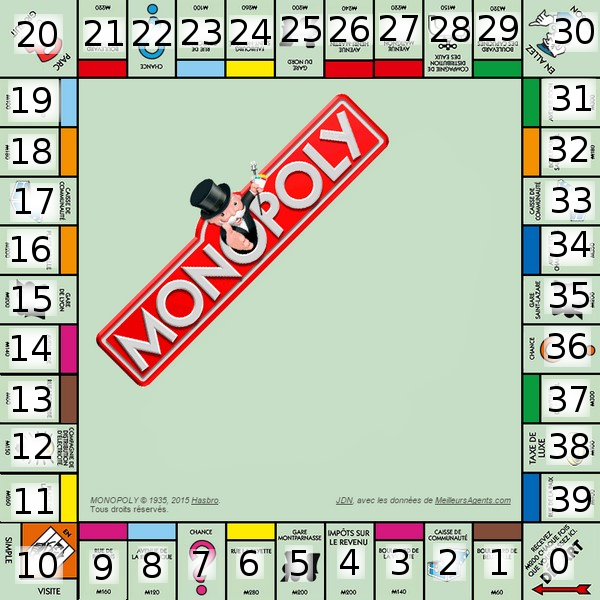
\includegraphics[scale=0.4]{./Images/Monopoly.png}
	\caption{Numéroation du Monopoly \citep{IMG_Monopoly}}
    \end{figure}
    
    Chaque déplacement du piont (c'est-à-dire à chaque fois que l'on lance le dé) sera 
    traduit par un changement d'état.
    Dans un premier temps, on modélise donc le Monopoly par 40 cases où chaque case est
    relié aux $6*n-(n-1)$ cases suivante à partir de la case $n-1$, où $n$ est le 
    nombre de dé.  Dans le cas précis des règles du Monopoly, chaque case pourra 
    donc accéder à 11 autres cases.  En effet, le résultat le plus petit pouvant être 
    produit par $n$ dés est de $n$ (tous les dé à 1).
    On devra donc élminer toutes les $n-1$ cases juste après la case actuelle et le résultat
    le plus grand pouvant être produit par $n$ dés est de $6*n$ (pour un dé à 6 faces).
    \begin{center}
      \begin{tikzpicture}
        \colornode[text width=1cm] at (0, 0) (c0) {Départ};
        \colornode[text width=0.7cm] at (1.5, 0) (c1) {Case 1};
        \colornode[text width=0.7cm] at (3, 0) (c2) {Case 2};
        \colornode[text width=1cm] at (5.5, 0) (cx) {...};
        \colornode[text width=0.7cm] at (7, 0) (c12) {Case 12};
        
        \drawedge
	  (c0) edge[bend left] node {} (c2)
	  (c0) edge[bend left] node {} (cx)
	  (c0) edge[bend left] node {} (c12)
	  (c1) edge[bend right] node {} (cx)
	  (c1) edge[bend right] node {} (c12);
        
      \end{tikzpicture}
    \end{center}
    Cependant, certaines cases ont un comportement particulier comme
    par exemple la case ``aller en prison'' sur laquelle on ne peut pas rester; en effet,
    celle-ci nous redirige directement dans la prison.  La case ``chance'' et ``caisse de
    communauté'' sont égalements des cas particuliers qui font que le Monopoly n'est pas 
    équiréparti.
    
  \subsection{Répartition des dés}
    \label{repart_des}
    Lorsque l'on lance $n$ dés, la somme des valeurs de chaque dés n'a pas la même probabilité
    d'apparaitre.  En effet, lorsque l'on lance 2 dés, il y a 3 manière différentes de formé
    un 4 (à savoir: $3+1$, $2+2$ et $1+3$) alors qu'il n'y a qu'une seule manière de formé un 
    2 (à savoir: $1+1$), comme illustré par la figure \ref{tableau_repartition_des}.
    \begin{figure}[h]
      \centering
      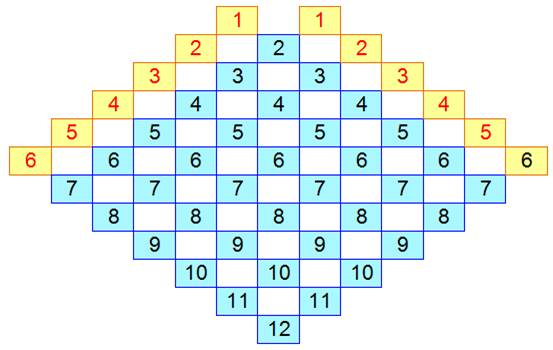
\includegraphics[scale=0.4]{./Images/RepartitionDes.jpg}
	\caption{Répartition des nombres formés avec 2 dés \citep{IMG_Des}}
      \label{tableau_repartition_des}
    \end{figure}
    Cette répartition peut être généralisé de la manière suivante:
    $$\sum\limits_{k=0}^{(s-n)/6} (-1)^k \begin{pmatrix}n \\ k\end{pmatrix} 
      \begin{pmatrix}s-6k-1 \\n-1\end{pmatrix}$$
    Source: %\url{http://villemin.gerard.free.fr/Wwwgvmm/Identite/Identxx2.htm\#formule}\\
    Où $n$ est le nombre de dés et $s$ le nombre que l'on désire former.  Cette equation
    a été construite suite à la décomposition en polynome permettant de calculer des
    réparition.\\
    En effet, en prennant par exemple le polynome $3x + 5x^2 + x^3$ et en le mettant au 
    carré, on va récupérer toutes les combinaissons possibles:
    \begin{align*}
     &(3x \times 3x) + (3x \times 5x^2) + (3x \times x^3) +\\
     &(5x^2 \times 5x^2) + (5x^2 \times x^3) + (x^3 \times x^3)\\
     &= (9x^2) + (15x^3) + (3x^4) + (25x^4) + (5x^5) + (x^6)\\
     &= x^6 + 5x^5 + 28x^4 + 15x^3 + 9x^2
    \end{align*}
    Ce calcul montre la répartition de dés truqués ayant 3 faces 1, 5 faces 2 et une face 3.
    Le résultat final nous montre que lorsque l'on lance 2 de ces dés de 9 faces. En faisant
    la somme des coefficients, on obtient le nombre d'arrangement possible.  Dans le cas
    présent, on a donc $1 + 5 + 28 + 15 + 9$ c'est à dire $59$.  Cela nous permet de dire
    qu'il y a une chance sur 59 que la somme de ses 2 dés forme un 6 et 28 chance sur 59
    de former un 4.\\
    L'équation exprimé au début de ce point représente simplement le développement de 
    ce polynome.
    % TODO Robin (remarque)
%     Le raisonnement sur les polynômes est assez clair, mais l'explication est un peu confuse : 
%     l'idée est d'utiliser les fonctions génératrices afin de trouver le nombre de combinaisons relatives à la somem des dés.
%     « Le résultat final nous montre que lorsque l’on lance 2 de ces dés de 9 faces. » La phrase n'est pas complète. ;)
    
  \subsection{Faire un double}
    % TODO un nombre indéfinit de dés... toujours un double où tous les dés les mêmes ?
    Les règles du Monopoly stipulent que lorsque l'on fait 3 doubles à la suite, on est
    envoyé en prison.  Pour modéliser ce comportement via une chaîne de Markov, il va 
    falloir triplé le nombre d'état.  En effet, une case $i$ peut être visité après avoir
    fait 0 double, 1 double ou 2 double.  Si de cette case $i$ on refaire encore un double,
    on se retrouve en case prison.  Si par contre on fait un simple nombre, on se retrouve
    de nouveau sur la case $i$ ``zero double''.  Il est assez simple de se rendre compte de
    ça via la figure \ref{representation_double}.  Sur cette image, on peut donc voir en 
    rouge les déplacements fait grace à des doubles.  Ces 3 lignes rouges montre
    donc le déplacement d'un joueur qui aurait lancé les dés et fait consécutivement 3 doubles,
    à savoir ici: $1+1$, $2+2$ et $6+6$.  Ce dernière double le conduit directement en prison.
    Les flèches bleus montrent ce qu'il se passe lorsque l'on fait un simple déplacement (pas un double).
    Elles vont toutes vers la même plateau (celui où on a encore fait zero double).
    \begin{figure}[h]
      \centering
      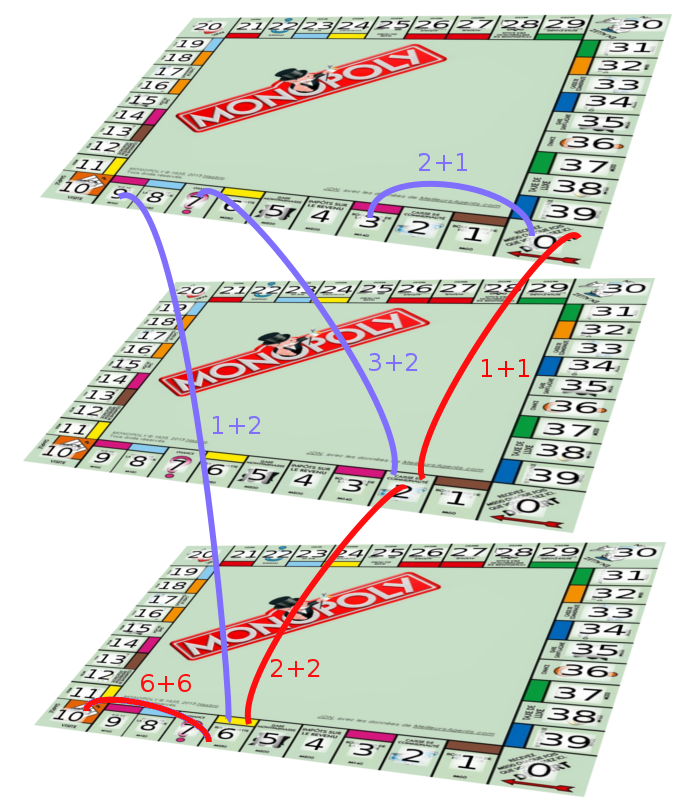
\includegraphics[scale=0.4]{./Images/MonopolyVertical.png}
	\caption{Déplacement en cas de double}
	\label{representation_double}
    \end{figure}
    % TODO question: lorsque l'on a fait 2 doubles et qu'on a une carte chance qui nous déplace... On a
    % toujours 2 doubles à notre actif ou pas ?
    Pour savoir si un nombre est un double, il suffit de vérifier que le nombre est divisible
    par le nombre de dés.  Il faut cependant bien tenir compte du fait qu'il y a plusieurs
    moyen de former un nombre.  Par exemple, avec deux dés, il y a trois manières différentes
    de former un 4: $1+3$, $2+2$ et $3+1$.  Il y a donc 3 chance sur 36 de faire un 4 mais
    seulement une sur 36 de faire un double et 2 sur 36 de faire un simple 4 avec deux dés
    différents.
    Dans le point % TODO
    
  \subsection{Case prison}
    \label{case_prison}
    Les règles du Monopoly stipulent que l'on peut sortir de prison de plusieurs manières 
    différentes: soit via une carte chance, soit en payant, soit en faisant un double.
    Seule les deux dernières solutions seront utilisé dans cette modélisation.  En effet,
    avoir une carte chance ne dépend pas uniquement de l'état précédent et ne peut donc
    pas être représenté facilement avec les chaînes de Markov. Les règles indiquent 
    également que l'on ne peut rester que 3 tours maximum avant d'être obligé de payer.
    Afin de représenter ces différentes cas, la case prison sera ``triplée``.  On aura
    donc trois représentations de la case prison: au premier, second et troisième tour.
    La case ''aller en prison`` sera donc considérée comme une case prison de niveau 0 et
    n'aura qu'une seule arrête visant la case ''prison premier tour``.
    Afin d'être le plus précis possible, on va calculer la probabilité de faire un double.
    Comme vu dans la \fullref{repart_des}, il y a 36 cas possible lorsque l'on lance 
    2 dés à 6 faces.  On sait qu'il y a 6 doubles.  On a donc 6 chance sur 36 de faire un
    double et chaque double: $2$, $4$, $6$, $8$, $10$ et $12$ ont chacun une chance sur 36
    d'apparaitre.  Si on ne fait pas de double (dans 5 cas sur 6), on doit relancer les 
    dés (et donc avant ça, passer à la case prison ''suivante``).
    Chaque case ''prison`` (les 3 cases cités ci-dessus) auront donc 8 arrêtes différentes:
    \begin{itemize}
     \item Payer et sortir de prison;
     \item Faire un double (et avancer du résultat de ce double), il y a donc 6 choix possibles;
     \item Ne pas réussir à faire un double (et continuer attendre).
    \end{itemize}
    
  \subsection{Case ''Chance``}
    Les cases chances peuvent faire gagner de l'argent mais également déplacé les pions 
    présent sur le plateau de jeu.  C'est évidemment ce second comportement qui sera
    étudier ici.  Le Monopoly comporte 16 cartes chances ayant la répartition suivante:
    \begin{itemize}
     \item 8 cartes faisant référence à des payements;
     \item une carte ''sortir de prison``;
     \item 7 cartes faisant référence à un déplacement.
    \end{itemize}
    On peut donc en déduire que lorsqu'un joueur pioche une carte chance, il aura une 
    7 chance sur 16 de devoir déplacer son pion.  Ces déplacements sont les suivants:
    \begin{itemize}
     \item Reculer de 3 cases;
     \item Se rendre à la case départ;
     \item Aller en prison;
     \item Se rendre à la 11ème case (où 0 est le départ);
     \item Se rendre à la 15ème case;
     \item Se rendre à la 24ème case;
     \item Se rendre à la 36ème case (dernière case avant l'arrivée).
    \end{itemize}
    Dans les 9 autres cas on lancera simplement les dés.  Les cases chances ont donc 
    beaucoup d'arrêtes.
    
  \subsection{Case ''Caisse de communauté``}
    Les cartes ''Caisse de communauté`` sont plus axé sur l'aspect financier du jeu.
    Cependant 3 cartes provoques également des déplacements des pions.
    \begin{itemize}
     \item Se rendre à la case départ;
     \item Aller en prison;
     \item Se rendre sur le première case.
    \end{itemize}
    La modélisation des cartes ''caisse de communauté`` se fait de la même manière que 
    les cartes ''Chance``.
    
  \subsection{Calcul de l'état stationnaire}
    Comme vu dans le point \ref{etat_stationnaire}, il est possible de calculer
    la distribution stationnaire de chaque case du Monopoly.  Pour se faire, on va
    se basé sur une des méthodes décrite dans ce même point, à savoir simplifier la
    fonction de base:
    \begin{align*}
     wP &= w\\
     wP &= wI\\
     w(P-I) &= 0
    \end{align*}
    Où $w$ est le vecteur stationnaire que l'on cherche, $P$ est la matrice de 
    déplacement et $I$ est la matrice identité.  On peut également noté cette 
    equation de la façon suivante:
    $$(P-I)^{T} w^{T} = 0$$
    Qui sera plus simple à implémenté dans un langage informatique.\\
    % TODO expliquer pourquoi ce sera plus simple (résolution linéaire)
    On peut également rajouter une colonne de 1 permettant d'intégrer directement la 
    contrainte suivante dans l'équation:
    $$\sum\limits_{i \in w} i = 1$$
    Cette équation part du simple principe que le vecteur résultat sera la distribution 
    de probabilité de chaque état.  Il faut donc que leur somme corresponde à 1 vu 
    que l'on exprime la probabilité de se trouver sur tous les états accèssibles, il y
    a donc une probabilié 1 de se trouver sur les états présent dans le vecteur résultat 
    (plus d'informations dans le point \ref{etat_stationnaire}).
    \paragraph{Avec un exemple concret}
    Prenons la matrice de déplacement suivante:
    % TODO exemple très mauvais !!!  Ce n'est pas une chaine de markov !
    \begin{align*} 
      wP = w\\ 
      % === NEW LINE ===
      % > w
      \left( 
	\begin{array}{ccc}
	w_1 & w_2 & w_3
	\end{array} 
      \right) 
      % > p
      \left( 
	\begin{array}{ccc}
	1 & 0 & 1 \\
	2 & 0 & 0 \\
	0 & 1 & 3 
	\end{array} 
      \right)
      = 
      % > w
      \left( 
	\begin{array}{ccc}
	w_1 & w_2 & w_3
	\end{array} 
      \right)  
      \\
      % === NEW LINE ===
      % w 
      \left( 
	\begin{array}{c}
	w_1\\
	w_2\\
	w_3
	\end{array} 
      \right)^T
      % (
      \left(
        % P
	\left(
	\begin{array}{ccc}
	1 & 0 & 1 \\
	2 & 0 & 0 \\
	0 & 1 & 3 
	\end{array} 
	\right)
	-
	% I
	\left(
	\begin{array}{ccc}
	1 & 0 & 0 \\
	0 & 1 & 0 \\
	0 & 0 & 1 
	\end{array} 
	\right)
      % )
      \right)
      = 0
      \\ 
      % === NEW LINE ===
      % w
      \left( 
	\begin{array}{ccc}
	w_1 & w_2 & w_3
	\end{array} 
      \right)
      % (P-I)
      \left( 
	\begin{array}{ccc}
	0 & 0 & 1 \\
	2 & -1 & 0 \\
	0 & 1 & 2 
	\end{array} 
      \right) 
      = 
      % 0
      \left( 
	\begin{array}{ccc}
	0 & 0 & 0
	\end{array} 
      \right)
      \\
      % === NEW LINE ===
      % (P-I)^T
      \left( 
	\begin{array}{ccc}
	0 & 0 & 1 \\
	2 & -1 & 0 \\
	0 & 1 & 2 
	\end{array} 
      \right)^T
      % w
      \left( 
	\begin{array}{c}
	w_1\\
	w_2\\
	w_3
	\end{array} 
      \right)
      = 
      % 0
      \left( 
	\begin{array}{c}
	0\\
	0\\
	0
	\end{array} 
      \right)
    \end{align*}
    On ajoute donc la colonne de 1:
    \begin{align*}
      \left( 
	\begin{array}{cccc}
	0 & 0 & 1 & 1 \\
	2 & -1 & 0 & 1 \\
	0 & 1 & 2 & 1
	\end{array} 
      \right)^T 
      \left( 
	\begin{array}{c}
	w_1\\
	w_2\\
	w_3
	\end{array} 
      \right)
      = 
      \left( 
	\begin{array}{c}
	0\\
	0\\
	0\\
	1
	\end{array} 
      \right)
    \end{align*}
    
    
  \subsection{Choix du langage}
    Pour modéliser le Monopoly, le langage Python a été choisi.  Il permet en effet
    d'avoir accès facilement à plusieurs librairies permettant de manipuler
    facilement des données.
    
    \subsubsection{Libraires utilisées}
      Pour manipuler plus facilement des matrices et résoudre les équations linéaire,
      la librairie ''numpy`` a été utilisé.  Concernant l'interface graphique, c'est
      la librairie ''Tkinter`` qui a été sélectionnée.
    
\section{Résultat}


\section{Conclusion}
  
  
%     ===== EXEMPLE =====
%     \begin{tikzpicture}
%       % Draw the states
%       \node[state,
% 	    text=yellow,
% 	    draw=none,
% 	    fill=gray!50!black] (s) {Sunny};
%       \node[state,
% 	    right=of s,
% 	    text=blue!30!white, 
% 	    draw=none, 
% 	    fill=gray!50!black] (r) {Rainy};
% 
%       % Connect the states with arrows
%       \draw[every loop]
% 	  (s) edge[bend right] node {} (r)
% 	  (r) edge[bend right] node {} (s)
% 	  (s) edge[bend right, auto=left]  node {0.6} (r)
% 	  (r) edge[bend right, auto=right] node {0.7} (s)
% 	  (s) edge[loop above]             node {0.4} (s)
% 	  (r) edge[loop above]             node {0.3} (r);
%     \end{tikzpicture}
  

\footnotesize
\bibliographystyle{apalike}
\bibliography{Rapport}


\end{document}